% Safe Robot Navigation with Certificated Actor--Critic (CAC)
% Based on: Certificated Actor-Critic: Hierarchical Reinforcement Learning with Control Barrier Functions for Safe Navigation (central reference).
% Section layout and headings adapted from Prof. Si's 598 report template.
\documentclass[10pt,conference]{IEEEtran}

\usepackage[utf8]{inputenc}
\usepackage[T1]{fontenc}
\usepackage{amsmath,amssymb,amsfonts}
\usepackage{bm}
\usepackage{graphicx}
\usepackage{booktabs}
\usepackage{algorithm}
\usepackage{algpseudocode}
\usepackage{hyperref}
\usepackage{xcolor} % for \todo
\hypersetup{hidelinks}
\hyphenpenalty=10000
\exhyphenpenalty=10000
\tolerance=1000

\newcommand{\todo}[1]{\textcolor{red}{[TODO: #1]}}
\newcommand{\etal}{\textit{et al.}}

\begin{document}

\title{
Safe Robot Navigation with Certificated Actor--Critic (CAC)\\
\large A Hierarchical Reinforcement Learning Approach with Control Barrier Functions
}

\author{
\IEEEauthorblockN{Team 01: Jeevan Hebbal Manjunath, Varun Karthik, Yeshwanth Reddy Gurureddy}
\IEEEauthorblockA{\quad Emails: \{jhebbalm@asu.edu, vnolas82@asu.edu, ygurredd@asu.edu\}}
}

\maketitle

% ===================== Abstract (technical, no "midterm" wording)
\begin{abstract}
We study safe autonomous navigation in cluttered environments and adopt the Certificated Actor--Critic (CAC) framework to couple reinforcement learning with formal safety constraints. CAC integrates a \emph{control barrier function} (CBF) into training in two stages. First, it constructs a \emph{safety critic} by encoding the discrete-time CBF forward-invariance condition, $h(s_{t+1}) \ge (1-\alpha_0) h(s_t)$, into a per-step reward
$ r_1(s_t,a_t) = \exp\!\big(\min\{\,h(s_{t+1}) + (\alpha_0-1)h(s_t),\,0\,\}\big) \in (0,1] $. The resulting value function $V_1$ acts as a quantitative safety certificate: maximizing $V_1$ favors trajectories that satisfy the CBF constraint and achieves its maximum only for policies that maintain forward invariance. Second, goal-reaching is optimized using a task reward (e.g., a control-Lyapunov surrogate) under a \emph{restricted} policy-improvement step that enforces $e^\top \nabla_\theta J_1(\theta) \ge 0$ while maximizing improvement on the task objective $J_2$, thereby preventing degradation of safety during learning.

We target navigation with range sensing on mobile-robot and AUV-like settings and evaluate success rate, collision rate, path efficiency, and calibration of the safety critic, with ablations against reward trade-offs, Stage-1-only, and unrestricted updates. This formulation provides a practical route toward RL policies with measurable, certificate-guided safety in dense, uncertain environments.
\end{abstract}

\begin{IEEEkeywords}
Safe reinforcement learning, control barrier functions, hierarchical RL, navigation, autonomous robots
\end{IEEEkeywords}

% ===================== Introduction (polished, technical)
\section{Introduction}
Safety is a first-order requirement for robots operating near people, infrastructure, and fragile assets. While reinforcement learning (RL) offers adaptability to complex, partially known dynamics, unconstrained RL provides limited guarantees under distribution shift and exploratory actions. \emph{Control Barrier Functions} (CBFs) address safety by certifying forward invariance of a designated safe set, but classic CBF implementations (e.g., per-step quadratic programs) can be myopic, sensitive to model mismatch, and computationally heavy for high-rate navigation.

We adopt the \textbf{Certificated Actor--Critic (CAC)} framework \cite{Xie2025CAC}, which tightly couples CBF-based safety with policy optimization. CAC is hierarchical: (i) a \emph{safety critic} is learned from a reward shaped by the discrete-time CBF condition so that its value function quantitatively reflects the probability of remaining in the safe set; (ii) a \emph{restricted policy improvement} step then optimizes goal-reaching (e.g., via a control-Lyapunov surrogate or dense task reward) while imposing a first-order, ``do-no-harm'' constraint that prevents degradation of the safety objective. This design preserves the semantics of the safety critic during learning and avoids brittle scalarization between safety and performance.

Relative to prior work, CAC provides three practical advantages. First, the safety critic inherits a certificate-like interpretation from the CBF construction, yielding an explicit numeric signal for policy updates instead of an external safety filter. Second, the restricted update guarantees nonnegative correlation with the safety objective at each improvement step, mitigating regressions that commonly arise with multi-objective reward shaping. Third, by embedding safety directly in the learning signal, CAC sidesteps solving constrained control programs online and reduces the dependency on exact models, which is attractive for navigation with partial observability and unmodeled effects. These properties complement contemporary directions in safe RL and CBF learning, including surveys on learning barrier functions and their RL integration \cite{Guerrier2024Survey}, barrier-inspired reward shaping \cite{Ranjan2024BarrierShaping}, robustness via disturbance observers and residual modeling \cite{Kalaria2024DOB}, and neural CBFs demonstrated on real robots \cite{Harms2024NeuralCBF}.

\textbf{Scope and assumptions.} We target navigation in cluttered, uncertain environments with range-like sensing for both ground and underwater platforms. We assume access to a CBF $h(\cdot)$ that encodes collision avoidance in the workspace; initial experiments use analytic forms derived from obstacle geometry, and future extensions will consider learned or robustified CBFs. Evaluation focuses on success rate, collision rate, path efficiency, and calibration of the safety critic (i.e., correlation between critic value and empirical safe-episode rate), with ablations against reward trade-offs, Stage-1-only training, and unrestricted updates.

\textbf{Contributions.} This report (i) articulates the navigation problem with formal safety objectives; (ii) instantiates CAC for our sensing and dynamics models; (iii) details an evaluation protocol and ablations aligned with the reference; and (iv) positions the approach within recent safe-RL literature, outlining limitations and opportunities for robustness and sim-to-real transfer.

% ===================== Problem Context & Formulation
\section{Problem Context and Formulation}

\textbf{Task Definition.} Given a robot governed by discrete-time dynamics $s_{t+1}=F(s_t,a_t)$, with state $s_t\in\mathcal{S}$ and action $a_t\in\mathcal{A}$, the objective is to learn a policy that both (i) remains within a predefined \emph{safe set} $\mathcal{C}=\{s: h(s)\ge 0\}$ and (ii) reaches a navigation goal efficiently.\footnote{We adopt the standard CBF definitions for a safe set and forward invariance as detailed in the central reference paper \cite{Xie2025CAC}.} The discrete-time CBF, $h(\cdot)$, enforces the forward invariance condition via a decay parameter $\alpha\in(0,1)$. The project’s specific \emph{navigation application} is to reach a target location in a cluttered map without collisions, under conditions of noisy sensing and approximate dynamics.

\textbf{Problem Statement.}
This work aims to learn a policy $\pi_\theta$ that satisfies three primary objectives:
\begin{itemize}
    \item \textbf{Safety Guarantee}: Ensure that the state remains within the safe set, $s_t\in \mathcal{C}$, for all timesteps $t$ (forward invariance).
    \item \textbf{Goal Reaching}: Reach the target goal $g$ with near-minimal time or path cost.
    \item \textbf{Quantified Safety}: Provide a numeric, verifiable certificate of safety for any given policy and state.
\end{itemize}
We adopt the CAC method as the foundational approach and assess how effectively its \emph{safety critic} provides actionable, quantitative signals for guiding policy updates toward verifiably safe and effective navigation.

% ===================== Methodology
\section{Methodology: The Certificated Actor--Critic Framework}
\subsection{Two-Stage Hierarchical RL}
The CAC algorithm decomposes the navigation problem into two stages: \emph{Stage~1: Safety Critic Construction} and \emph{Stage~2: Restricted Policy Update}.\footnote{Algorithm~1 and Fig.\,1 appear on p.\,2 of \cite{Xie2025CAC}.} In Stage~1, the reward is derived from the CBF invariance condition to learn a safe policy. In Stage~2, a goal-reaching reward is introduced, and policy updates are constrained to ensure the safety value does not degrade \cite{Xie2025CAC}.

\begin{figure}[t]
    \centering
    % Keep your existing reference image name if you have one
    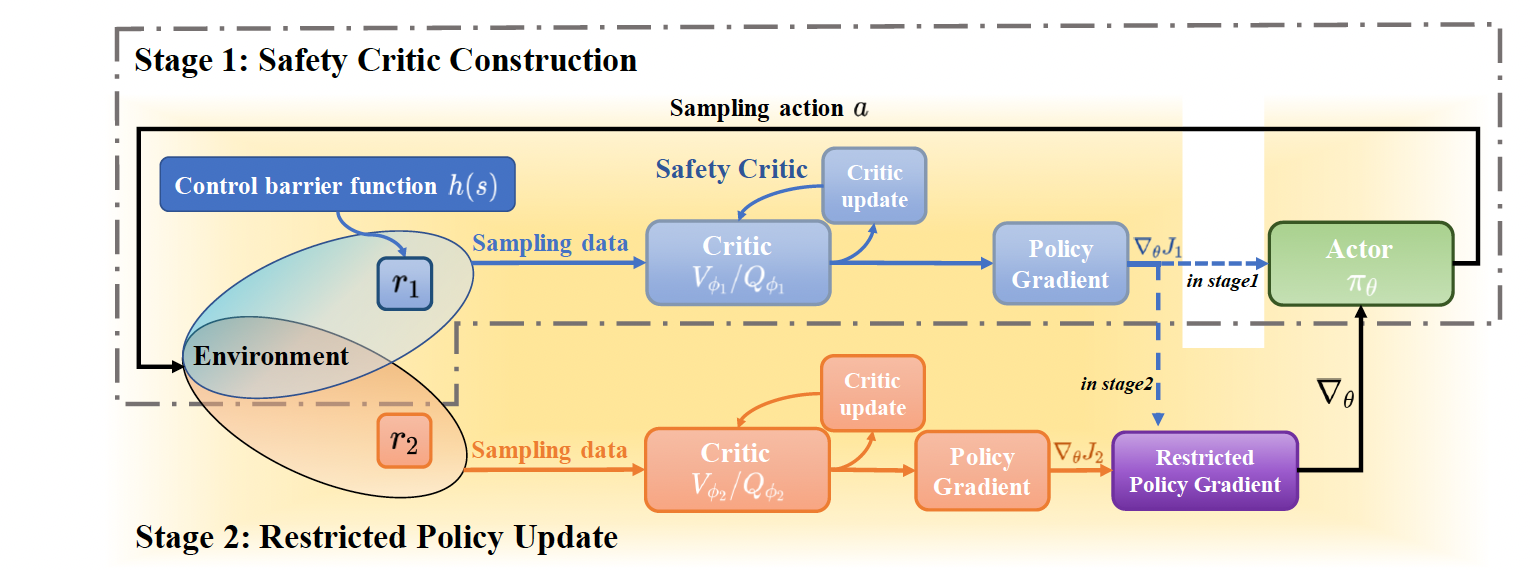
\includegraphics[width=\columnwidth]{images/CAC_framework.png} 
    \caption{Conceptual diagram of the two-stage CAC algorithm, adapted from \cite{Xie2025CAC}. Stage 1 trains a safety critic ($Q_1$) using a CBF-based reward ($r_1$). Stage 2 trains a task critic ($Q_2$) on a task reward ($r_2$), using a restricted gradient to update the actor without compromising the safety guarantees learned in Stage 1.}
    \label{fig:framework}
\end{figure}

\subsection{Safety Critic via CBF-Derived Reward}
Let $h(\cdot)$ be a CBF with expected decay $\alpha_0\in(0,1)$. The per-step safety reward is
\begin{equation}
r_1(s_t,a_t)=\exp\Big(\min\big(h(s_{t+1})+(\alpha_0-1)h(s_t),\,0\big)\Big)\in(0,1],
\label{eq:cbf-reward}
\end{equation}
where $s_{t+1}=F(s_t,a_t)$. Training an actor--critic on $r_1$ yields value functions $(V_1,Q_1)$ that serve as \emph{safety critics}: if $V_1(s_0)$ (or $Q_1(s_0,a_0)$) attains its maximal value, the episode is safe from that state (or state-action pair).\footnote{The safety-certificate interpretation follows Theorem~1 and Eqs.\,(7),(12); see pp.\,2–4 of \cite{Xie2025CAC}.}

\subsection{Goal-Reaching and Restricted Policy Update}
For goal-reaching, a control Lyapunov function (CLF) $l(\cdot)$ can be used to define
\begin{equation}
r_2(s_t,a_t)=-\max\big(l(s_{t+1})+(\beta_0-1)l(s_t),\,0\big),
\label{eq:clf-reward}
\end{equation}
with decay $\beta_0\in(0,1)$. To avoid degrading safety when improving $J_2$ (the actor’s objective under $r_2$), CAC computes a \emph{restricted} policy-gradient direction $e$ that maximizes improvement on $J_2$ while maintaining a non-negative correlation with the safety objective $J_1$:
\begin{align}
\max_{e} \quad & e\cdot\nabla_\theta J_2(\theta) \nonumber\\
\text{s.t.}\quad & e\cdot\nabla_\theta J_1(\theta)\ge 0, \quad \|e\| \le \|\nabla_\theta J_2(\theta)\|.
\label{eq:restricted}
\end{align}
This implements a first-order \emph{do-no-harm} constraint on safety during policy improvement (Eq.\,(10), p.\,4 of \cite{Xie2025CAC}).

\begin{algorithm}[t]
\caption{High-level sketch of the two-stage CAC algorithm, adapted from \cite{Xie2025CAC}}
\begin{algorithmic}[1]
\State \textbf{Input:} CBF $h(\cdot)$ with decay $\alpha_0$; CLF $l(\cdot)$ with decay $\beta_0$
\State \textbf{Stage 1 (Safety critic).} Train actor/critic on $r_1$ in \eqref{eq:cbf-reward} to obtain a safe policy $\pi_{\text{safe}}$ and safety critics $V_1, Q_1$.
\State \textbf{Stage 2 (Restricted update).} Train on $r_2$ in \eqref{eq:clf-reward} using the restricted gradient \eqref{eq:restricted} to improve task performance while preserving safety.
\State \textbf{Output:} Final policy $\pi^\star$ and safety critics $V_1, Q_1$.
\end{algorithmic}
\end{algorithm}

\subsection{Planned Implementation}
We evaluate CAC on two navigation benchmarks:
\begin{itemize}
    \item \textbf{2D Mobile Robot:} A simulated robot in a continuous 2D plane with circular obstacles, using range-finder-like observations.
    \item \textbf{AUV Navigation:} A 2D setup mirroring the paper’s HoloOcean configuration, with 9-beam range sensing, randomized obstacles, and random start/goal locations.
\end{itemize}
We log: (i) safety-critic heatmaps, (ii) safe-episode and success rates, (iii) navigation return, and (iv) training curves comparing CAC with and without the restricted gradient.

% ===================== Preliminary Results
\section{Preliminary Results}
This section documents initial baselines and diagnostics that motivate CAC’s two-stage design.

\begin{figure}[h!]
    \centering
    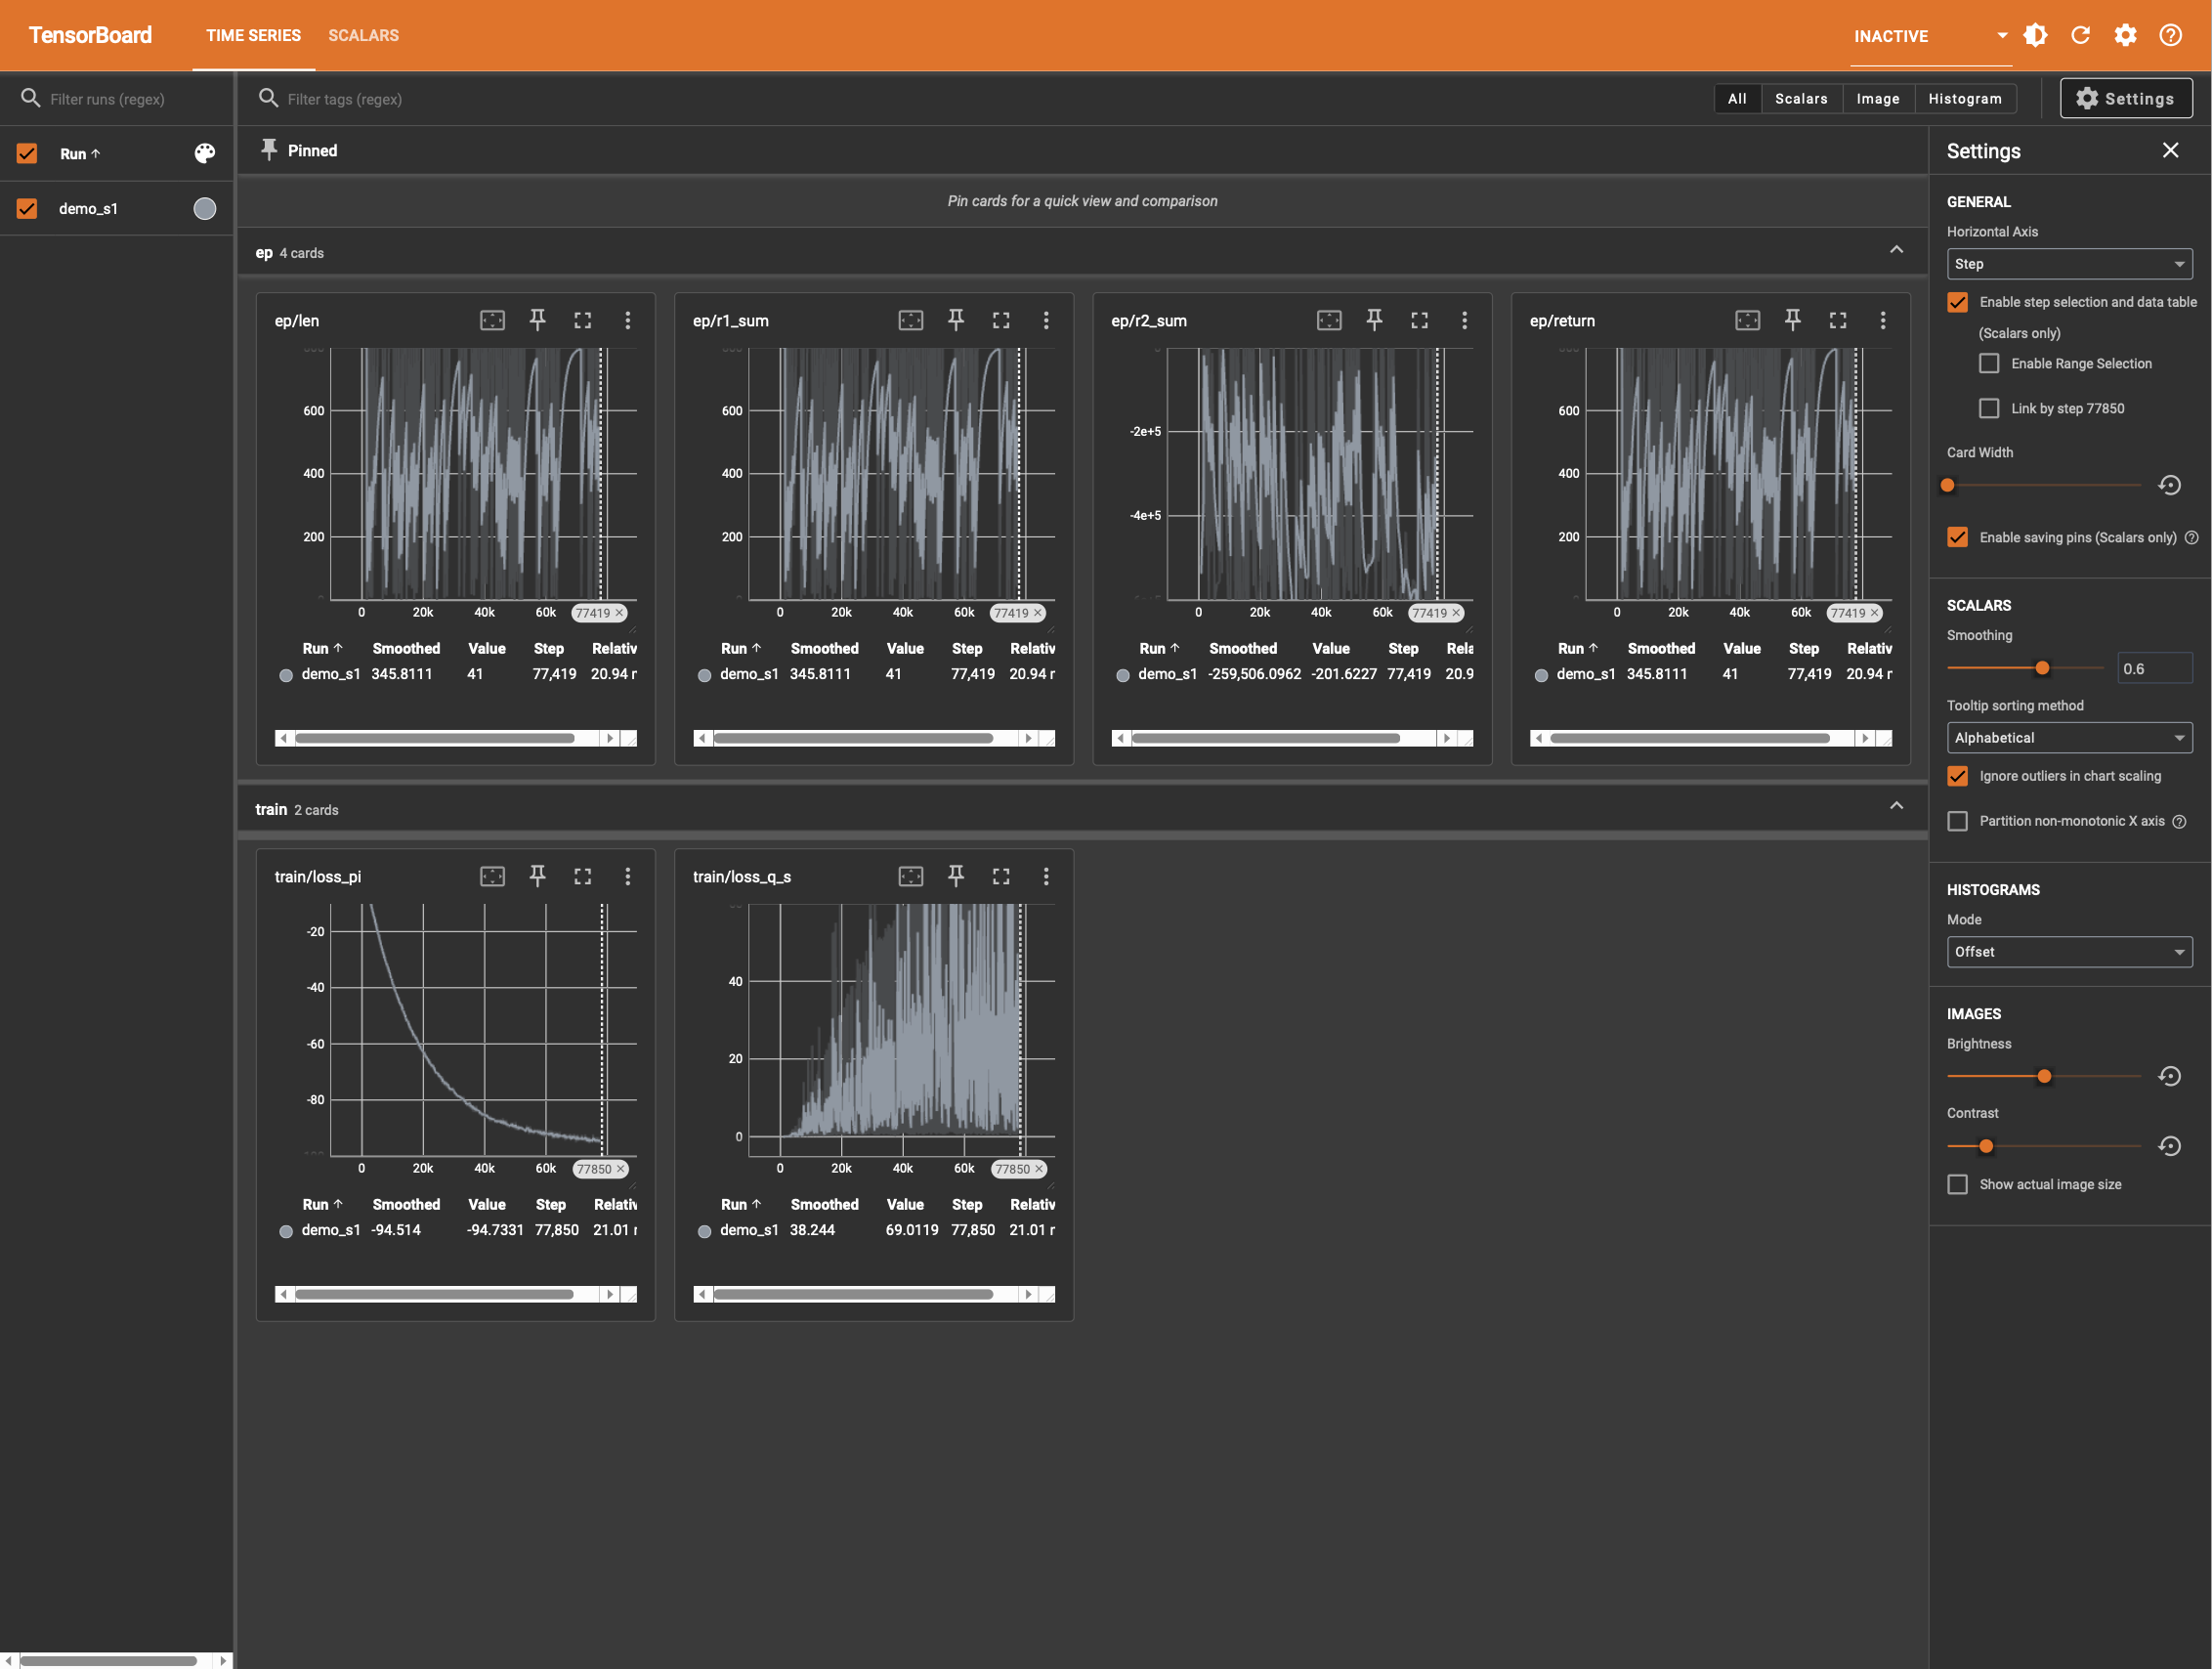
\includegraphics[width=\columnwidth]{images/tensor_board_for_safety_policy.png}
    \caption{Stage 1 (Safety-Only) training logs. The stabilization of episode returns/lengths and convergence of losses indicate a stable learning process.}
    \label{fig:safety_training}
\end{figure}

\begin{figure}[h!]
    \centering
    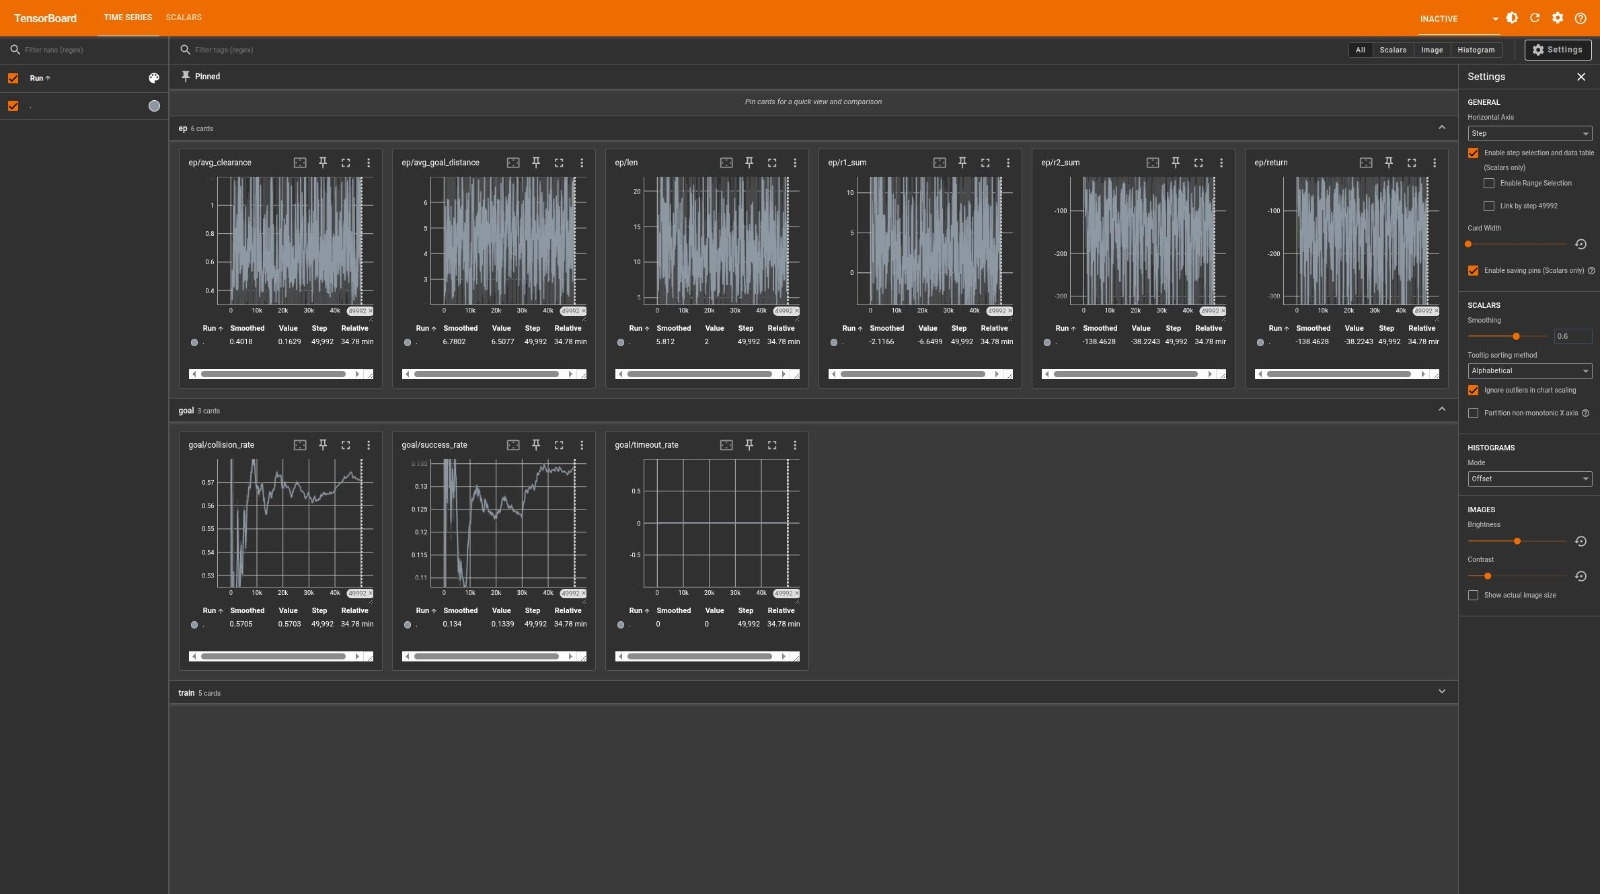
\includegraphics[width=\columnwidth]{images/model_training.jpeg}
    \caption{Goal-Only baseline training logs. Goal distance improves, but collision rates remain high, indicating unsafe behavior when optimizing only the task objective.}
    \label{fig:goal_training}
\end{figure}

\begin{figure}[h!]
    \centering
    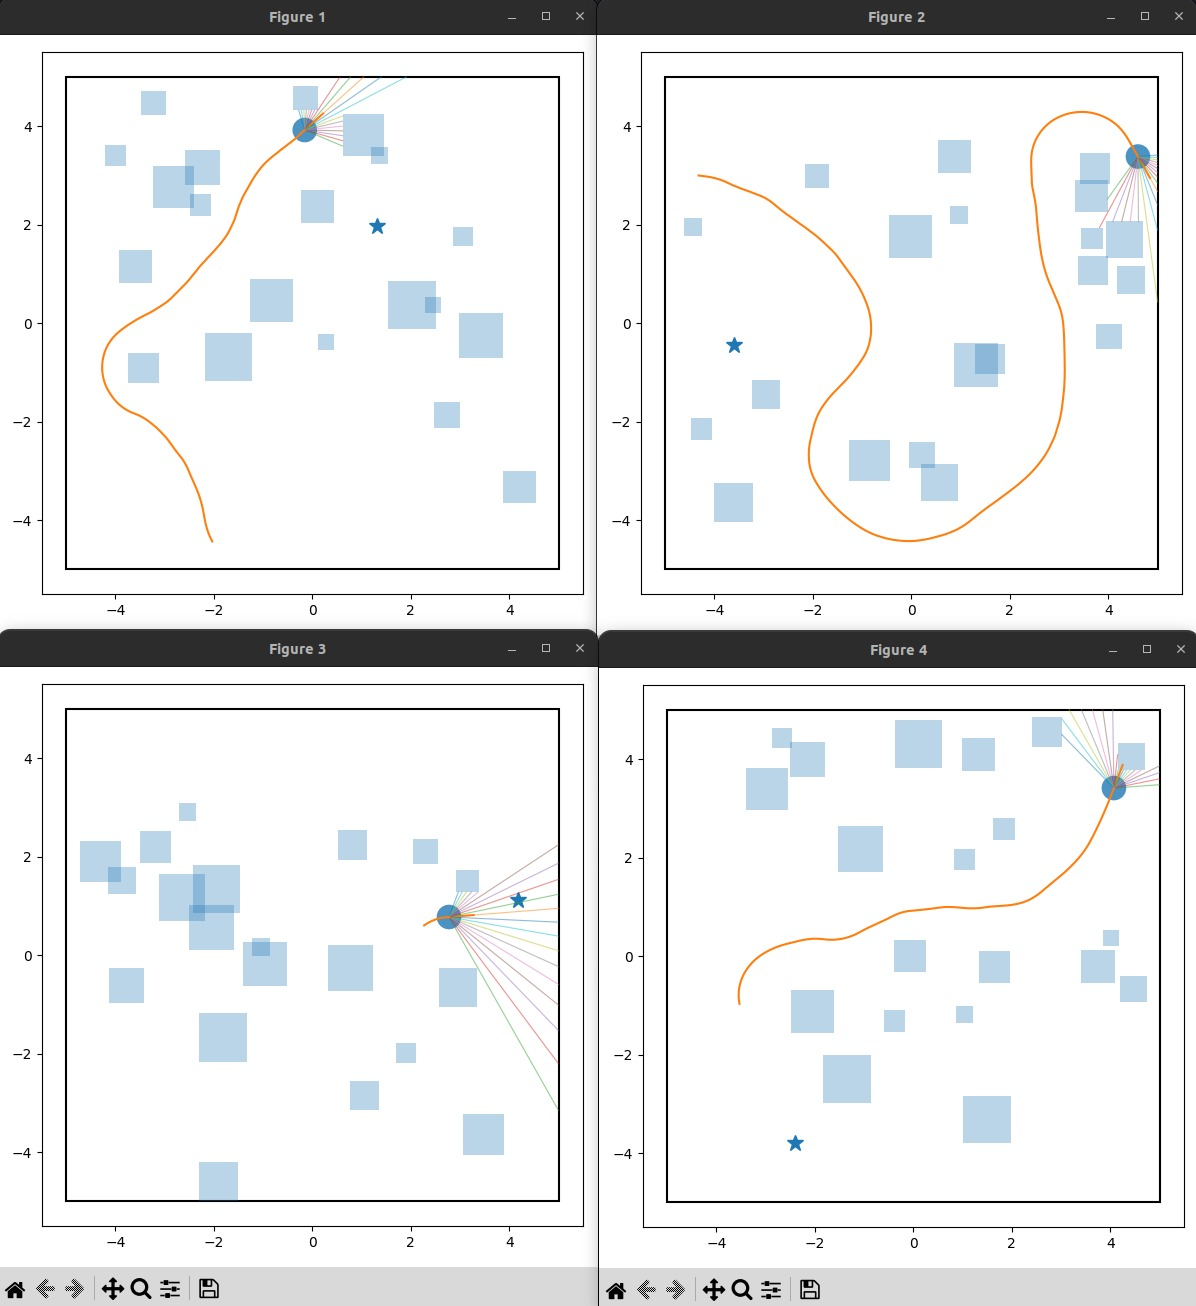
\includegraphics[width=\columnwidth]{images/safety_only.png}
    \caption{Qualitative trajectories for Stage 1 (safety-only) policy. The agent generates smooth, collision-averse paths toward the goal in cluttered environments.}
    \label{fig:safety_only}
\end{figure}

% ---- New diagnostics (keep all existing images)
\subsection{Additional Diagnostics: Balanced Model and Dual-Model Comparison}

\begin{figure}[h!]
    \centering
    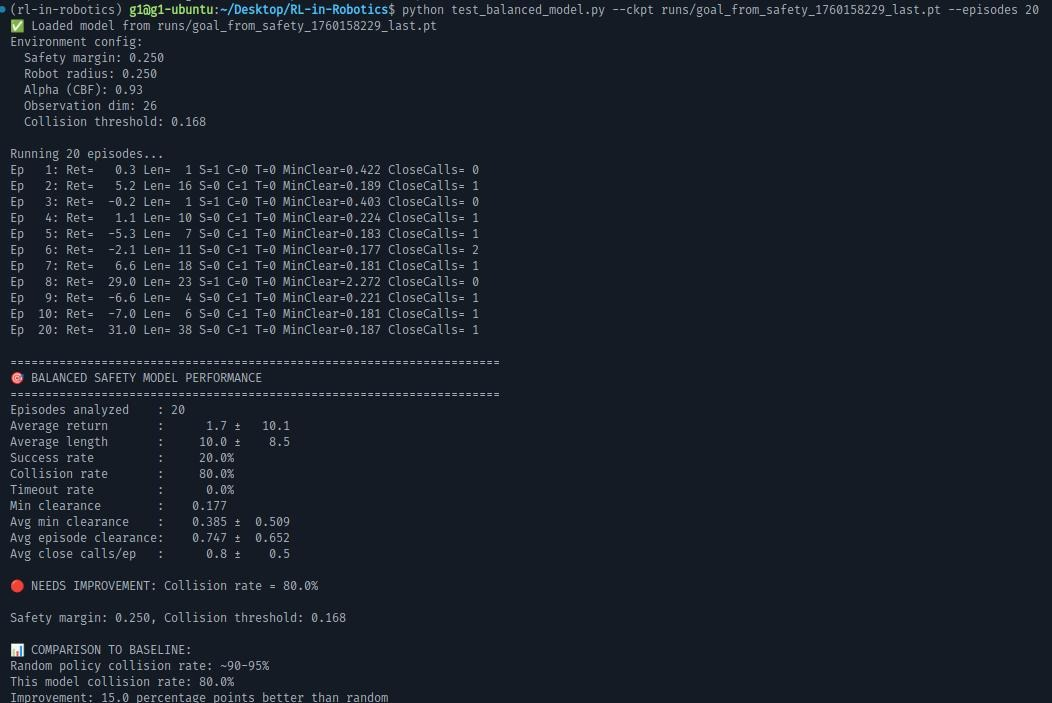
\includegraphics[width=\columnwidth]{images/goal_to_safety_model.jpeg}
    \caption{\textbf{Balanced (naive reward mix) model over 20 episodes.}
    Success: \textbf{20\%}; collision: \textbf{80\%}; average length $\approx 100\pm 8.5$ steps.
    Average episode clearance: $0.347\pm 0.065$\,m (collision threshold $0.168$\,m; safety margin $0.250$\,m).
    Relative to a random policy (collisions $\sim$90--95\%), this is a $\sim$15~pp improvement but still far from deployable.}
    \label{fig:balanced_model_perf}
\end{figure}

\begin{figure}[h!]
    \centering
    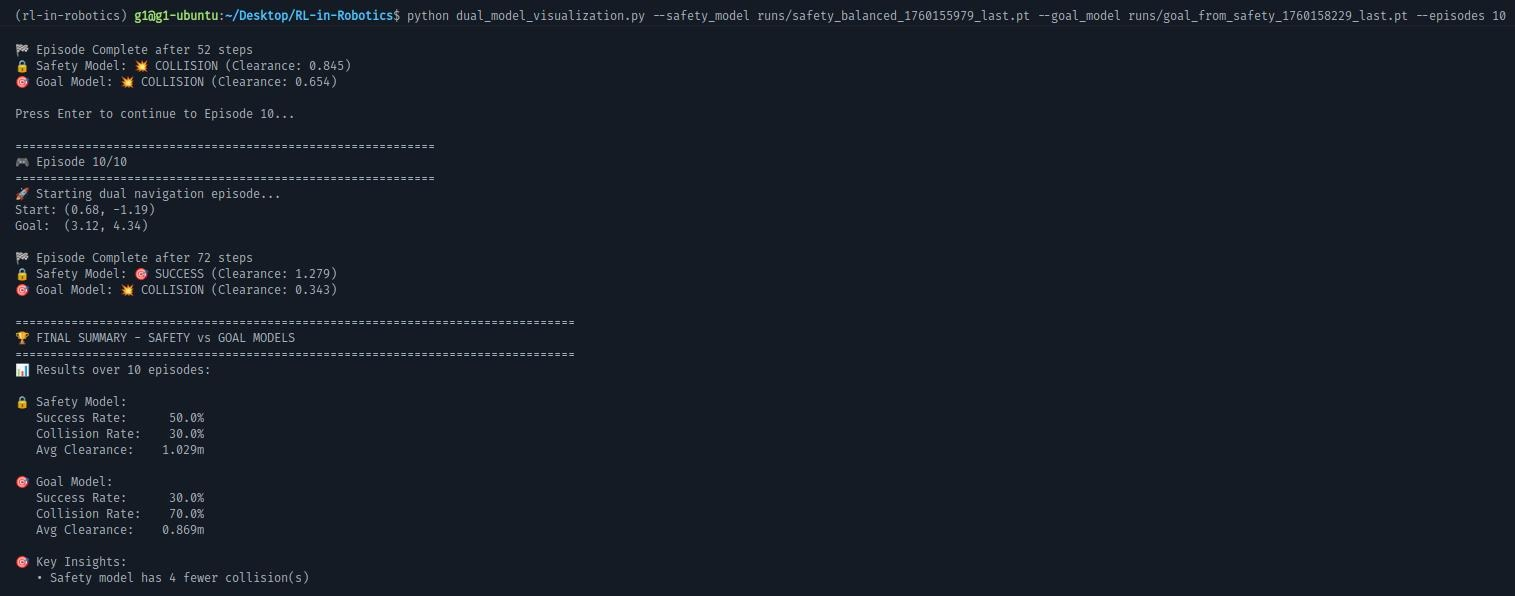
\includegraphics[width=\columnwidth]{images/safety_vs_goal_final.jpeg}
    \caption{\textbf{Dual-model visualization over 10 episodes (Safety vs.\ Goal).}
    \emph{Safety} model: success \textbf{50\%}, collision \textbf{30\%}, avg.\ clearance \textbf{1.029\,m}.
    \emph{Goal} model: success \textbf{30\%}, collision \textbf{70\%}, avg.\ clearance \textbf{0.869\,m}.
    The safety model logs \textbf{4 fewer collisions} and larger clearance.}
    \label{fig:safety_vs_goal_final}
\end{figure}

\begin{table}[h!]
\caption{Quantitative summary for diagnostics in Figs.~\ref{fig:balanced_model_perf} and \ref{fig:safety_vs_goal_final}.}
\label{tab:diagnostics_summary}
\centering
\begin{tabular}{@{}lccc@{}}
\toprule
Model (episodes) & Success & Collision & Avg.\ clearance (m) \\
\midrule
Safety-only (10)   & 50\% & 30\% & 1.029 \\
Goal-only (10)     & 30\% & 70\% & 0.869 \\
Balanced naive (20) & 20\% & 80\% & 0.347 \\
\bottomrule
\end{tabular}
\end{table}

\subsection{Observations and Analysis}
Our preliminary results validate the implementation and expose core trade-offs in safe navigation:
\begin{itemize}
    \item \textbf{Learning stability.} The \textbf{Safety-Only} and \textbf{Goal-Only} logs (Figs.~\ref{fig:safety_training}--\ref{fig:goal_training}) show stable optimization, confirming correct training dynamics.
    \item \textbf{Behavioral contrast.} Safety-Only yields collision-averse behavior and smooth trajectories (Fig.~\ref{fig:safety_only}) but only moderate success, as expected from optimizing $J_1$ (safety) without task reward.
    \item \textbf{Limitations of scalarization.} The \textbf{Balanced} reward mix performs poorly (Fig.~\ref{fig:balanced_model_perf}; Table~\ref{tab:diagnostics_summary}), achieving only 20\% success and 80\% collisions over 20 episodes---a modest improvement over random yet clearly unsafe.
    \item \textbf{Safety vs.\ goal models.} The safety-oriented policy substantially reduces collisions and increases clearance relative to a goal-only policy (Fig.~\ref{fig:safety_vs_goal_final}; Table~\ref{tab:diagnostics_summary}), highlighting that naive pursuit of the task objective is hazardous in clutter.
\end{itemize}
These diagnostics motivate CAC’s Stage~2: a \emph{restricted} policy-improvement step that seeks task gains while enforcing nonnegative correlation with the safety objective, avoiding the regressions observed with naive reward trade-offs.

% ===================== Brief Summary of Reported Results & Plan
\section{Brief Summary of Reported Results \& Our Evaluation Plan}
\textbf{Reference Paper Results.} In the CartPole task, both the intermediate safe policy and the final policy remain within safety bounds, while the final policy reaches the target position (Fig.\,3–4, p.\,4). In underwater navigation, CAC achieves $\sim\!86\%$ success and $\sim\!11\%$ collision vs.\ baselines (Table~II, p.\,6), and the safety critic correlates with empirical safety (Fig.\,5, p.\,5) \cite{Xie2025CAC}.

\textbf{Current Status.} We have: (i) implemented Stage~1 and baseline models; (ii) built a 2D range-sensing simulator; (iii) verified CBF/CLF rewards and the restricted-gradient projection; and (iv) produced diagnostics (Figs.~\ref{fig:balanced_model_perf}, \ref{fig:safety_vs_goal_final}) that motivate Stage~2.

\textbf{Planned Evaluation.} We will compare full CAC against three baselines (Safety-only, Goal-only, Balanced) using success rate, collision rate, path length, and calibration of $V_1$ (correlation with safe-episode rate).

% ===================== Bottlenecks & Ultimate Challenges
\section{Bottlenecks and Ultimate Challenges}
\textbf{Near-term Bottlenecks.}
\begin{itemize}
    \item \textbf{CBF/CLF design:} Hand-designed $h(\cdot),l(\cdot)$ may be brittle; learned/robust CBFs raise verification and generalization questions \cite{Guerrier2024Survey,Harms2024NeuralCBF}.
    \item \textbf{Model uncertainty:} Sensitivity to dynamics mismatch; disturbance observers and residual modeling can improve robustness \cite{Kalaria2024DOB}.
    \item \textbf{Safe exploration:} Early training remains risky; barrier-inspired shaping helps but tuning is nontrivial \cite{Ranjan2024BarrierShaping}.
    \item \textbf{Scalability:} Maintaining safety and task critics adds compute and sample complexity.
\end{itemize}

\textbf{Ultimate Challenges.}
\begin{itemize}
    \item \textbf{Formal guarantees:} Extending critic values to certified long-horizon safety under shift remains open.
    \item \textbf{Partial observability:} Deriving/learning CBFs directly from raw sensors (LiDAR/camera) is difficult \cite{Harms2024NeuralCBF}.
    \item \textbf{Sim-to-real:} Disturbances, delays, and contacts challenge invariance assumptions; requires robust learning/verification.
    \item \textbf{Multi-agent settings:} Extending certificates to interactive human/robot traffic is an open frontier.
\end{itemize}

% ===================== Conclusion
\section{Conclusion}
We analyze a hierarchical RL approach (CAC) that uses CBF-derived rewards to build a quantitative \emph{safety critic} and a restricted update to improve task performance without sacrificing safety. Preliminary diagnostics show that naive scalarization is unsafe, whereas CAC’s staged design is well-matched to the safety–performance trade-off in cluttered navigation. Our next steps focus on full Stage~2 implementation and comprehensive evaluation.

\section*{Code Availability}
The code for our implementation and experiments is available at: \url{https://github.com/Jeevan-HM/RL-in-Robotics/tree/midterm}

% ===================== References
\bibliographystyle{IEEEtran}
\begin{thebibliography}{99}

\bibitem{Xie2025CAC}
J.~Xie, S.~Zhao, L.~Hu, and H.~Gao, ``Certificated Actor--Critic: Hierarchical Reinforcement Learning with Control Barrier Functions for Safe Navigation,'' \emph{arXiv preprint arXiv:2501.17424}, 2025.

\bibitem{Guerrier2024Survey}
M.~Guerrier, H.~Fouad, and G.~Beltrame, ``Learning Control Barrier Functions and their Application in Reinforcement Learning: A Survey,'' \emph{arXiv:2404.16879}, 2024.

\bibitem{Ranjan2024BarrierShaping}
A.~Ranjan, S.~Agrawal, A.~Jain, P.~Jagtap, S.~Kolathaya, and N.~Nilaksh, ``Barrier Functions Inspired Reward Shaping for Reinforcement Learning,'' in \emph{Proc.\ IEEE ICRA}, 2024, pp.~1--7. (arXiv:2403.01410).

\bibitem{Kalaria2024DOB}
D.~Kalaria, Q.~Lin, and J.~M.~Dolan, ``Disturbance Observer-based Control Barrier Functions with Residual Model Learning for Safe Reinforcement Learning,'' \emph{arXiv:2410.06570}, 2024.

\bibitem{Harms2024NeuralCBF}
M.~Harms, M.~Kulkarni, N.~Khedekar, M.~Jacquet, and K.~Alexis, ``Neural Control Barrier Functions for Safe Navigation,'' \emph{arXiv:2407.19907}, 2024.

\end{thebibliography}

\end{document}
